%%%%%%%%%%%%%%%%%%%%%%%%%%%%%%%%%%%%%%%%%%%%%%%%%%%%%%%%%%%%%%%%%%%%%%%%
%    INSTITUTE OF PHYSICS PUBLISHING                                   %
%                                                                      %
%   `Preparing an article for publication in an Institute of Physics   %
%    Publishing journal using LaTeX'                                   %
%                                                                      %
%    LaTeX source code `ioplau2e.tex' used to generate `author         %
%    guidelines', the documentation explaining and demonstrating use   %
%    of the Institute of Physics Publishing LaTeX preprint files       %
%    `iopart.cls, iopart12.clo and iopart10.clo'.                      %
%                                                                      %
%    `ioplau2e.tex' itself uses LaTeX with `iopart.cls'                %
%                                                                      %
%%%%%%%%%%%%%%%%%%%%%%%%%%%%%%%%%%
%
%
% First we have a character check
%
% ! exclamation mark    " double quote  
% # hash                ` opening quote (grave)
% & ampersand           ' closing quote (acute)
% $ dollar              % percent       
% ( open parenthesis    ) close paren.  
% - hyphen              = equals sign
% | vertical bar        ~ tilde         
% @ at sign             _ underscore
% { open curly brace    } close curly   
% [ open square         ] close square bracket
% + plus sign           ; semi-colon    
% * asterisk            : colon
% < open angle bracket  > close angle   
% , comma               . full stop
% ? question mark       / forward slash 
% \ backslash           ^ circumflex
%
% ABCDEFGHIJKLMNOPQRSTUVWXYZ 
% abcdefghijklmnopqrstuvwxyz 
% 1234567890
%
%%%%%%%%%%%%%%%%%%%%%%%%%%%%%%%%%%%%%%%%%%%%%%%%%%%%%%%%%%%%%%%%%%%
%
\documentclass[10pt]{iopart}
\newcommand{\gguide}{{\it Preparing graphics for IOP Publishing journals}}
%Uncomment next line if AMS fonts required
%\usepackage{iopams} 
\usepackage{graphicx}
\usepackage{cite}
\begin{document}

\title[]{Energy Transfer in a Type-I van der Waals Heterostructure of WSe$_2$/PtSe$_2$}

\author{Pengzhi~Wang$^{1,2,3}$,
                Yongsheng~Wang$^{2}$,
                Ang~Bian$^{2}$,
				Shengcai~Hao$^{4,5}$,
                Qing~Miao$^{2}$,
                Xiaoxian~Zhang$^{2}$,
                Jiaqi~He$^{1,*}$,
                Dawei~He$^{2,*}$ and Hui~Zhao$^{6,*}$}
\address{$^{1}$College of Mathematics and Physics\unskip, Beijing University of Chemical Technology\unskip, Beijing\unskip, 100029\unskip, China}
\address{$^{2}$Key Laboratory of Luminescence and Optical Information, Ministry of Education, Institute of Optoelectronic Technology\unskip, Beijing Jiaotong University\unskip, Beijing\unskip, 100044\unskip, China}
\address{$^{3}$GBA branch of Aerospace Information Research Institute\unskip, Chinese Academy of Sciences\unskip,  Guangzhou\unskip, 510700\unskip, China}
\address{$^{4}$Beijing Institute of Electro-machining Co.,Ltd.\unskip, Beijing Key Laboratory of Electro Discharge Machining Technology\unskip, Beijing\unskip, 100191\unskip, China}
\address{$^{5}$Beijing Academy of Science and Technology\unskip, Beijing\unskip, 100089\unskip, China}
\address{$^{6}$Department of Physics and Astronomy\unskip, The University of Kansas\unskip, Lawrence\unskip, Kansas\unskip, 66045\unskip, USA}
\ead{jqhe@buct.edu.cn; dwhe@bjtu.edu.cn; huizhao@ku.edu}

\vspace{10pt}
\begin{indented}
\item[]March 2022
\end{indented}

\begin{abstract}
Energy transfer of a van der Waals heterostructure formed by monolayers of WSe$_2$ and PtSe$_2$ is studied by steady-state photoluminescence and time-resolved transient absorption spectroscopy. The heterostructure sample is fabricated by transferring a mechanically exfoliated WSe$_2$ monolayer onto a PtSe$_2$ monolayer film obtained by chemical vapor deposition. The sample is thermally annealed to improve the interface quality. Photoluminescence of the heterostructure is quenched by 4 times compared to the individual WSe$_2$ monolayer, indicating excitation transfer from WSe$_2$ to PtSe$_2$. Femtosecond transient absorption measurements with two configurations show that both the electrons and the holes can transfer from WSe$_2$ to PtSe$_2$ on a sub-picosecond time scale, while neither can transfer from PtSe$_2$ to WSe$_2$. These results indicate that WSe$_2$ and PtSe$_2$ monolayers form a type-I band alignment with both the conduction band minimum and the valence band maximum in the PtSe$_2$ layer. 
\end{abstract}

%
% Uncomment for keywords
\vspace{2pc}
\noindent{\it Keywords}: PtSe$_2$, van der Waals
heterostructure, energy transfer, transient absorption spectroscopy

%
% Uncomment for Submitted to journal title message
\submitto{\TDM}
%
% Uncomment if a separate title page is required
%\maketitle
% 
% For two-column output uncomment the next line and choose [10pt] rather than [12pt] in the \documentclass declaration
\ioptwocol
%

\section{Introduction}

Two-dimensional (2D) materials, such as graphene\cite{geim2007rise}, transition metal dichalcogenides (TMDs)\cite{splendiani2010emerging,mak2010atomically}, hexagonal boron nitride\cite{song2010large}, and phosphorene\cite{wang2014two,hu2018two,lin20162d},  have been extensively studied in recent years due to their interesting physical properties originated from their nanoscale thickness. Besides their potential applications as individual materials\cite{zhang2014electrically},  these 2D materials can be stacked together to form artificial materials with tailored properties. With weak van der Waals interaction, this approach can combine different 2D materials in heterostructures with high interface quality and emergent properties \cite{xia2017recent}, which can have wide applications in photodetection\cite{yu2013highly},  photovoltaic\cite{britnell2013strong,furchi2014photovoltaic},  and light-emitting devices\cite{cheng2014electroluminescence}.

The heterostructures formed by two monolayer materials can have different types of energy band alignments, which allow sophisticated control of charge carriers. Figure \ref{fig:alignment} shows schematically typical band alignments and excitation transfer processes between two monolayers\cite{bellus2017type}.  Assuming that layer 1 has a larger band gap than layer 2, a type-I band alignment can form if the conduction band minima (CBM) and the valence band maxima (VBM) of the two materials are both in layer 2. The F{\"o}rster-type energy transfer can occur {\it via} dipole-dipole coupling of the two materials, where an electron-hole pair (or exciton) in layer 1 recombines, transferring the energy for the excitation of an electron-hole pair (or exciton) in layer 2 [Figure \ref{fig:alignment}(a)]\cite{hoeben2005supramolecular}.   The type-I band alignment also allows energy transfer {\it via} the Dexter mechanism by sequential or simultaneous transfer of both carriers [Figure \ref{fig:alignment}(b)]\cite{dexter1953theory,murphy2004probing}. In both cases, there is no net charge transfer between the two layers. When the CBM and the VBM are in different layers, as shown in Figure \ref{fig:alignment}(c)-\ref{fig:alignment}(d), a type-II band alignment is formed, which can drive interlayer charge transfer carried by either the electrons (c) or the holes (d), resulting in the layer-separated charge carriers. 

\begin{figure}[ht]
    \centering
    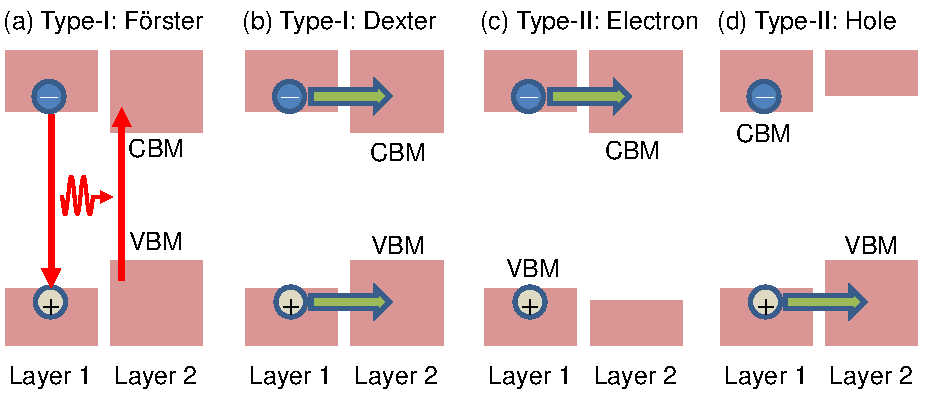
\includegraphics[width=8cm]{alignment.pdf}
    \caption{Band alignments and excitation transfer processes showing F{\"{o}}rster-type (a) and Dexter-type energy transfer (b) in type-I band alignments, and electron (c) and hole transfer (d) in type-II band alignments.}
    \label{fig:alignment}
\end{figure}

Recent studies have revealed that the band alignments of most van der Waals heterostructures formed by 2D semiconductors are type-II. For example, all 6 heterostructures formed by the most commonly studied TMD semiconductors, MoS$_2$, WS$_2$, MoSe$_2$, and WSe$_2$, have type-II band alignments\cite{hong2014ultrafast,ceballos2014ultrafast,bellus2015tightly,fang2014strong,gong2015two,kumar2018interlayer},  which allow efficient interlayer charge transfer and separation. These features are beneficial for optoelectronic applications such as photovoltaic devices and photodetectors since the spatial separation of the electrons and holes often results in extended carrier lifetimes. However, the type-I band alignment is suitable for light emission applications since the electrons and the holes are confined in the same layer, facilitating their efficient radiative recombination. So far, however, only a few type-I semiconducting 2D heterostructures have been discovered, including MoS$_2$/ReS$_2$\cite{bellus2017type},  WSe$_2$/MoTe$_2$\cite{li2018type,bae2021light},  and PbI$_2$/WS$_2$\cite{zheng2019probing}.  Hence, developing new type-I heterostructures could expand application of such elusive artificial materials in light-emitting applications.

Here we show that a newly developed 2D semiconductor, PtSe$_2$\cite{wang2021layered},   provides  opportunities to construct type-I heterostructures. Very recently, high-quality 2D films of PtSe$_2$ have been produced by mechanical exfoliation\cite{zhao2017high,ciarrocchi2018thickness,yu2018atomically,liang2019high,szydlowska2020spectroscopic},  chemical vapor deposition\cite{wang2016facile,yim2016high,shi2019chemical,hu2019unveiling}, molecular beam epitaxy\cite{yan2017high},   and Pt film selenization\cite{wang2015monolayer,yao2017direct,o2016raman}.  Monolayer PtSe$_2$ with a distorted 1$T$ lattice \cite{wang2015monolayer,o2016raman,lin2017intrinsically} is semiconducting with an indirect bandgap of 1.2 eV \cite{zhao2017high,wang2015monolayer,guo2016biaxial,xie2019optical} and moderate charge mobilities\cite{zhao2017high,yang2019homogeneous}.  Its application, as an individual material, in various devices has been studied, such as field-effect transistors\cite{zhao2017high,urban2020isotropic},  photovoltaic devices\cite{yim2016high},  and photodetectors\cite{zhao2017high,yu2018atomically,liang2019high,yim2016high,su2018phase,yim2018wide,long2020scalable,yang2021high,luo2019pdse2,wang2020high,wang2020bound}.  In this work, a monolayer PtSe$_2$ is combined with a monolayer WSe$_2$ to form a heterostructure. Steady-state and time-resolved optical measurements on its photocarrier dynamics reveal efficient energy transfer from WSe$_2$ to PtSe$_2$ with absence of net charge transfer. The experimental results establish WSe$_2$/PtSe$_2$ as a type-I heterostructure with novel energy transfer properties.

\section{Experimental}
Monolayer PtSe$_2$ samples are acquired from 6 Carbon Technology Corporation, which are synthesized by chemical vapor deposition on c-cut sapphire substrates. Monolayer WSe$_2$ flakes are mechanically exfoliated from a bulk crystal (acquired from 2D Semiconductors). A dry-transfer technique is used to stack a WSe$_2$ flake on top of a PtSe$_2$ film.  Another monolayer WSe$_2$ flake is transferred onto a bare c-cut sapphire substrate for comparison. The samples are annealed at 200$^\circ$C for 8 hours in 2 Torr Ar environment to improve their interface quality. 

Raman and photoluminescence (PL) spectroscopy measurements are performed with a LabRAM HR Evolution Raman spectrometer (Horiba Jobin Yvon), using a continuous-wave excitation source of 532 nm. The differential reflection measurements are done with an ultrafast laser system (Newport) composed of a Ti:sapphire laser (80 MHz, 820 nm, and 100 fs), an optical parametric oscillator, and a harmonic-generation unit.  A homemade microscope in horizontal configuration is combined with the laser system\cite{bian2020dynamics}.  In such measurements, a tightly focused pump pulse excites the sample. The differential reflectance of a probe pulse, which arrives at a controllable delay time with respect to the pump pulse, is measured. The differential reflectance is defined as $\Delta R/R_0 = (R-R_0)/R_0$, where $R$ and $R_0$ are the probe reflectance with and without the pump, respectively.

 \section{Results and Discussion} 
 The crystal model of the heterostructure formed by monolayers of WSe$_2$ and PtSe$_2$ is shown in the upper panel of Figure \ref{fig:sample}(a). Monolayer WSe$_2$ has transport and optical band gaps of 2.00 and 1.63 eV, respectively\cite{he2014tightly},  both of which are much larger than the 1.2-eV band gap of PtSe$_2$ \cite{zhao2017high,wang2015monolayer,guo2016biaxial,xie2019optical}. Hence, if the band alignment of this heterostructure is type-I, both the CBM and the VBM are in the PtSe$_2$ layer, as illustrated in the lower panel of Figure \ref{fig:sample}(a). A type-II band alignment could form if either the CBM or the VBM of PtSe$_2$ is out of the forbidden band of WSe$_2$. Our experimental results, to be presented below, however, support the type-I alignment. Figure \ref{fig:sample}(b) shows an optical microscope image of the heterostructure sample, where a monolayer WSe$_2$ flake (outlined by the black dashed line) is transferred onto a continuous film of monolayer PtSe$_2$ on a sapphire substrate. The lateral size of the heterostructure region is on the order of 10 $\mu$m, which is sufficient for optical measurements. Another monolayer WSe$_2$ flake is transferred to a bare substrate, as shown in Figure \ref{fig:sample}(c), for comparison measurements.

\begin{figure}[ht!]
  \centering
  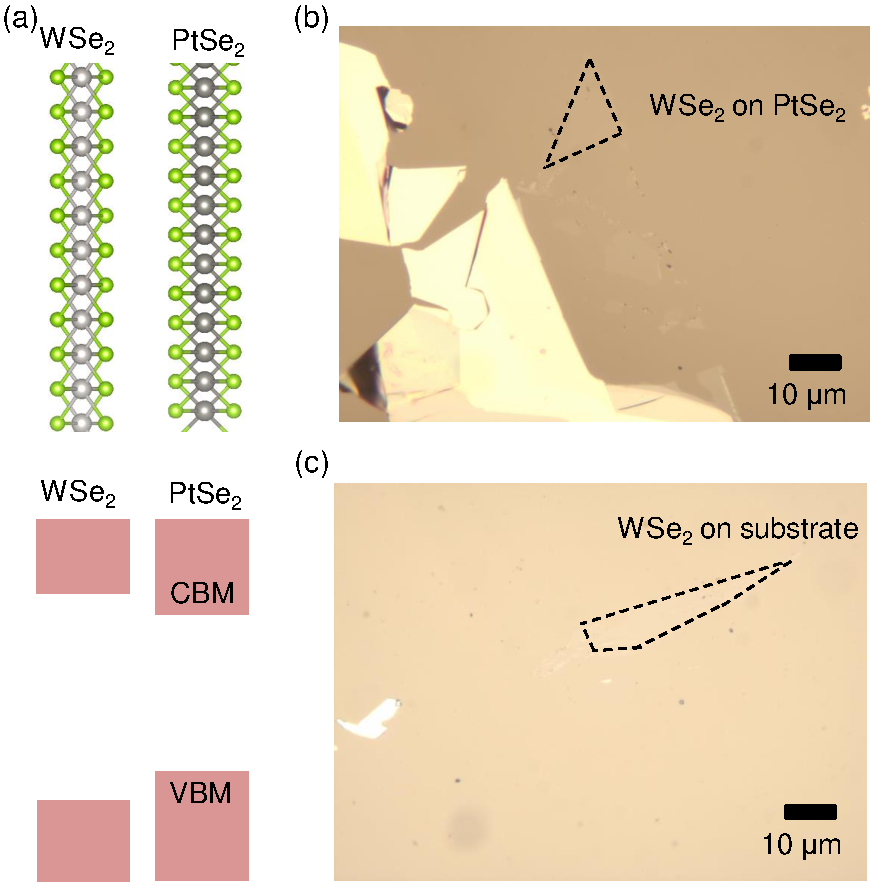
\includegraphics[width=8cm]{sample.pdf}
  \caption{(a) Crystal model (top) and schematics of type-I band alignment of the WSe$_2$/PtSe$_2$ heterostructure. (b) and (c) Optical microscope images of the heterostructure and monolayer WSe$_2$ samples, respectively.}
    \label{fig:sample}
\end{figure}



Figure \ref{fig:pl}(a) shows the Raman spectra of the WSe$_2$ (black) and PtSe$_2$ monolayers (red) and that of their heterostructure (blue) under 532-nm excitation. From WSe$_2$, the two peaks near 250 cm$^{-1}$ are consistent with previously reported $E_{2g}^1$ and A$_{1g}$ modes of WSe$_2$ monolayers\cite{gu2019layer,zhao2013lattice}. 
 The two main peaks at 181 cm$^{-1}$ and 209 cm$^{-1}$ from PtSe$_2$ are from the $E_g$ and $A_{1g}$ modes, respectively\cite{szydlowska2020spectroscopic,yim2016high}.  Furthermore, the intensity ratio of the $A_{1g}$ to $E_g$ peaks is about 7.6 \%, which  confirms its monolayer thickness\cite{szydlowska2020spectroscopic}.  The small feature at about 230 cm$^{-1}$ is identified as the longitudinal optical (LO) mode\cite{o2016raman}.  In the heterostructure sample, Raman features of both monolayers are observed. Hence, these measurements confirm the monolayer thickness of the PtSe$_2$ and WSe$_2$ samples.



Photoluminescence (PL) spectroscopy is performed to probe the sample quality and the potential charge or energy transfer processes. As shown by the black curve in Figure \ref{fig:pl}(b), the PL from the WSe$_2$ monolayer under the excitation of 532 nm shows a narrow peak at about 1.67 eV, which is consistent with its monolayer thickness\cite{ceballos2017separating}.  This peak in the heterostructure sample is quenched by about a factor of 4, as shown by the blue curve, under the same experimental condition. This indicates that photocarriers excited in the WSe$_2$ layer of the heterostructure sample have an additional efficient decay channel compared to those in the individual WSe$_2$ layer. Previous studies on 2D heterostructures have shown that charge transfer (of electrons or holes) and energy transfer can often provide such a channel\cite{ceballos2014ultrafast,fang2014strong,ceballos2015probing}. Hence, the PL quenching observed confirms the high interface quality of the sample and the existence of either energy or charge transfer in this heterostructure. No PL signal is detected from the monolayer PtSe$_2$ in this spectral range, which is reasonable considering its band gap of 1.2 eV.

\begin{figure}[ht!]
  \centering
  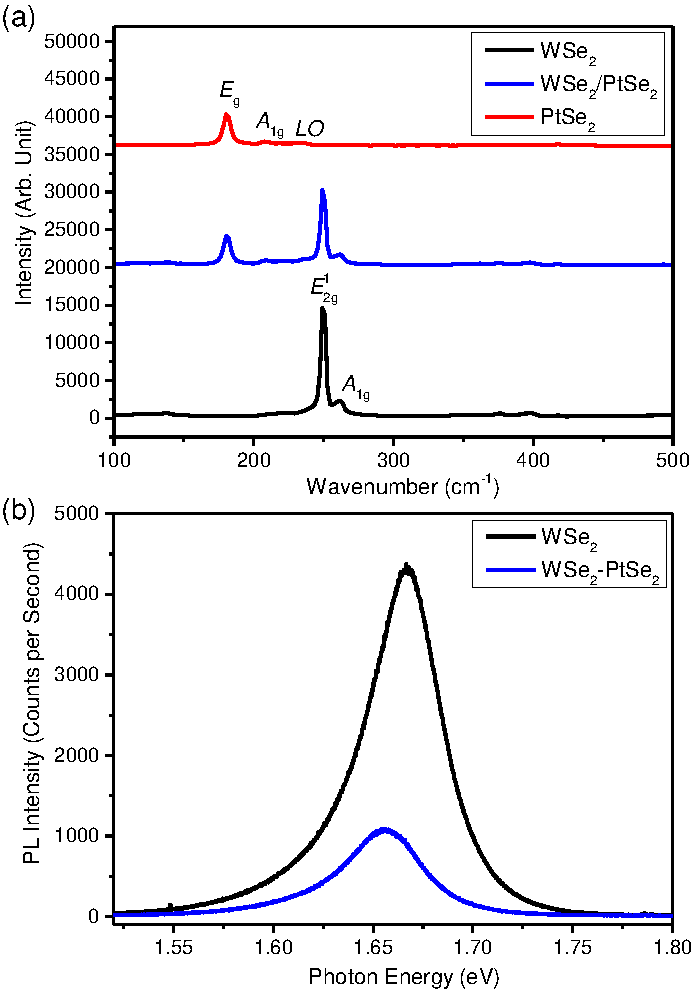
\includegraphics[width=8cm]{pl.pdf}
  \caption{(a) Raman spectra of the WSe$_2$/PtSe$_2$ heterostructure and the individual monolayer WSe$_2$ and PtSe$_2$ samples under the same experimental conditions. (b) Photoluminescence spectra of the WSe$_2$/PtSe$_2$ heterostructure and the monolayer WSe$_2$ samples under the same experimental conditions.}
    \label{fig:pl}
\end{figure}

To probe the photocarrier dynamics and interlayer excitation transfer, transient absorption measurements are performed in reflection geometry, using a 3.02-eV pump and a 1.67-eV probe pulses, as schematically shown in Figure \ref{fig:410743}(a). We first discuss the control measurement performed on the individual WSe$_2$ monolayer sample, as shown by the black squares in Figure \ref{fig:410743}(b) and \ref{fig:410743}(c) for short and long time scales, respectively. The pump pulse has an energy fluence of 2.7 $\mu$J cm$^{-2}$, corresponding to a photon density of $5.6 \times 10^{12}$ cm$^{-2}$ per pulse and an injected carrier density of $5.6 \times 10^{11}$ cm$^{-2}$ according to an absorbance of about 0.1 at this photon energy\cite{li2014measurement}. The rise of the signal can be fit by the integral of a Gaussian function with a full width at half maximum of 0.38 ps (dashed line). Since both the pump and the probe pulses are broadened to about 0.25 ps at the sample, due to the dispersive optical elements (mainly a microscope objective lens), the expected time resolution of the setup is 0.36 ps. Hence, the observed rise time is close to the instrumental limit, indicating that the pump-injected photocarriers produce a peak signal on a time scale much shorter than the resolution. This observation is consistent with previous results on WSe$_2$ \cite{cui2014transient} and other TMD monolayers\cite{nie2014ultrafast}. After the peak, the decay of the signal can be fit by a biexponential function, $\Delta R/R_0 (t) = A_1 \mathrm{exp}(-t/\tau_1) + A_2 \mathrm{exp}(-t/\tau_2) +A_0$, as shown by the black solid curves in Figure \ref{fig:410743}(b) and \ref{fig:410743}(c). The $\tau_1$ $(0.56 \pm 0.08$ ps) process accounts for 74\% of the total signal, which is due to the formation of the excitons from the pump-injected electron-hole pairs, according to previous studies\cite{ceballos2016exciton,steinleitner2017direct}. The $\tau_2$ $(46 \pm 5$ ps), which accounts for  21\% of the signal, is due to the nonradiative recombination of the excitons\cite{nie2014ultrafast,yan2014photoluminescence}.  There is a 5\% background, which is likely due to the trapped excitons by defects. 

\begin{figure*}[ht]
  \centering
  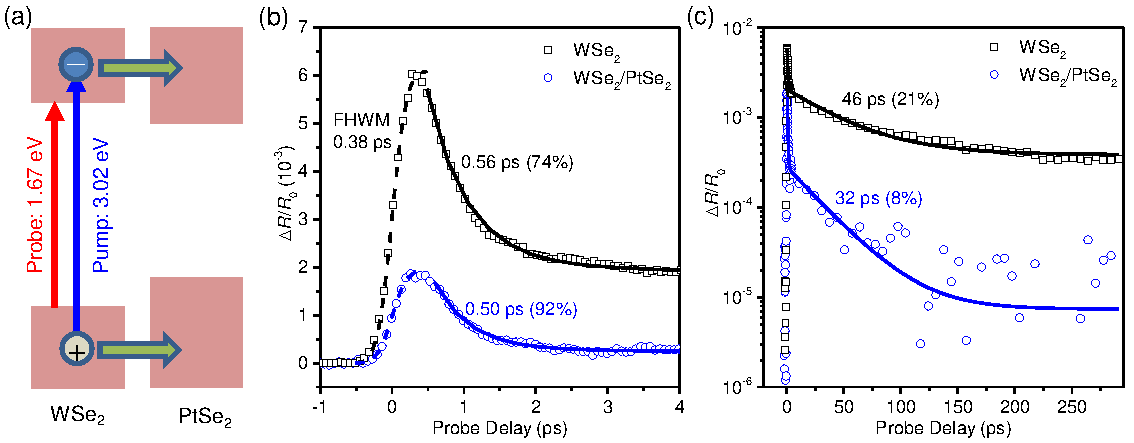
\includegraphics[width=16cm]{410743.pdf}
  \caption{(a) Schematics of the pump-probe measurement with 3.02-eV pump and 1.67-eV probe pulses. (b) and (c) Time dependent differential reflectance signal on short and long time ranges, respectively, for the WSe$_2$ monolayer (black) and the WSe$_2$/PtSe$_2$ heterostructure samples (blue). The curves are fits (see text).}
    \label{fig:410743}
\end{figure*}

The blue circles in Figure \ref{fig:410743} show the results of the same measurement performed on the WSe$_2$/PtSe$_2$ heterostructure sample. The signal rises to peak on the same 0.38 ps time scale [blue dashed curve in Figure \ref{fig:410743}(b)], followed by a fast decay process of $\tau_1 = 0.5 \pm 0.1$ ps (92\%) and a slow decay process of  $\tau_2 = 32 \pm 5$ ps (8\%). The significant difference of the two signals shown in Figure \ref{fig:410743} is strong evidence of the type-I band alignment of the WSe$_2$/PtSe$_2$ heterostructure with efficient energy transfer from WSe$_2$ to PtSe$_2$. First, we can rule out a lack of interfacial excitation transfer process due to, for example, a poor interface or insufficient band offsets. If that was the case, one would expect the same results from the two measurements, since in both cases the signal would be from the photocarriers that are injected in WSe$_2$ by the pump and subsequentially recombine there. The PtSe$_2$ layer of the heterostructure would have no effect on these photocarriers in WSe$_2$. Second, we can rule out a type-II band alignment. In a type-II alignment, the CBM and VBM are in different layers. As shown in Figure \ref{fig:alignment}(c)-\ref{fig:alignment}(d), such an alignment would drive transfer of one type of the photocarriers (electrons or holes) to PtSe$_2$, leaving the other type in WSe$_2$. This charge transfer process would separate the electrons and the holes to the two layers, forming long-lived interlayer excitons. In this case, the signal from the heterostructure should have a slow-decay component due to the long lifetime of the carriers (electrons or holes) in WSe$_2$\cite{peng2016ultrafast,wang2016interlayer}. Previous studies have shown that the interlayer excitons in type-II van der Waals heterostructures can produce a sizable and long-lived transient absorption signal at the intralayer exciton resonances of the individual layers, since these exciton states are formed by superposition of the conduction band and valence band states\cite{ceballos2014ultrafast,hong2014ultrafast}. However, most of the signal of the heterostructure (92\%) decays in 0.5 ps, indicating the lack of the layer-separated photocarriers.

The features observed from the heterostructure are consistent with a type-I band alignment. We assign the fast rise and the fast decay of the signal to sub-picosecond transfer of both electrons and holes from WSe$_2$ to PtSe$_2$. The lower peak signal of the heterostructure, compared to the individual WSe$_2$ monolayer, suggests that the transfer is {\it via} Dexter mechanism \cite{dexter1953theory,murphy2004probing} achieved by sequential transfer of electrons and holes [Figure \ref{fig:alignment}(b)]. Due to the expected large VB offset, the holes could transfer with a time much shorter than the rise time of the signal, and hence would manifest itself as a reduction of the peak signal due to loss of hole population in WSe$_2$ during the signal rise process. The 8\% signal that decays on 32 ps time scale could be attributed to parts of the sample with poor interface, whereas the photocarriers excited do not transfer. This part of the sample behaves as monolayer WSe$_2$. Hence, its signal also has a fast decay component due to exciton formation, as we observed in monolayer WSe$_2$. Therefore, the 0.5-ps decay process observed in the heterostructure sample has contributions from the exciton formation in this part of the sample as well as electron transfer from the rest of the sample.

The measurement on the heterostructure sample is repeated with various pump fluences, as shown in Figure \ref{fig:power}(a). The peak signal is proportional to the pump fluence, and thus the injected carrier density [Figure \ref{fig:power}(b)]. This feature confirms that the signal is proportional to the carrier density. By biexponential fits, as described above, the fast decay constant increases with decreasing the pump fluence, as shown in Figure \ref{fig:power}(c). This feature suggests that the interlayer transfer time of the slower carriers (likely the electrons) increases with lower carrier density. Considering that the transfer of these electrons is partially driven by the Coulomb force from the transferred holes in PtSe$_2$, this feature could be attributed to the weaker field with lower charge density. The slow decay time constant, $\tau_2$, is independent of the pump fluence (not shown).


\begin{figure}[ht!]
  \centering
  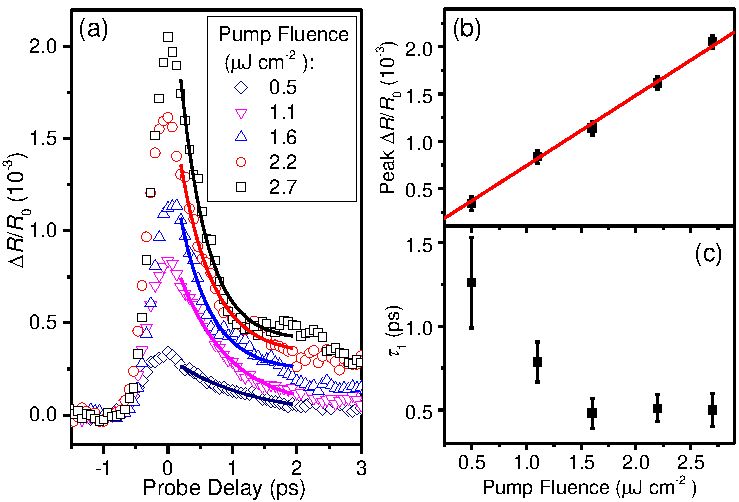
\includegraphics[width=8cm]{power.pdf}
  \caption{(a) Differential reflectance of the 1.67-eV probe from the WSe$_2$/PtSe$_2$ heterostructure sample under various fluences of the 3.02-eV pump pulse. Solid curves are fits. (b) and (c) The peak signal and the fast decay constant ($\tau_1$) as a function of the pump fluence, respectively.}
    \label{fig:power}
\end{figure}

\begin{figure*}[ht!]
  \centering
  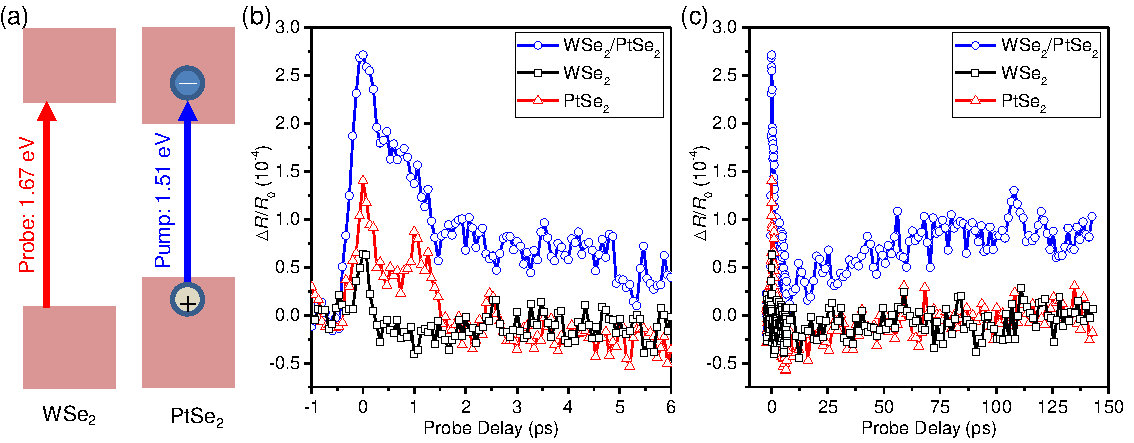
\includegraphics[width=16cm]{820743.pdf}
  \caption{(a) Schematics of the pump-probe measurement with 1.51-eV pump and 1.67-eV probe pulses. (b) and (c) Time dependent differential reflectance signal on short and long time ranges, respectively, for WSe$_2$ monolayer (black), WSe$_2$/PtSe$_2$ heterostructure (blue), and PtSe$_2$ monolayer (red).}
    \label{fig:820743}
\end{figure*}

To further confirm the type-I band alignment of the WSe$_2$/PtSe$_2$ heterostructure, another pump-probe configuration is used, as shown in Figure \ref{fig:820743}(a). The 1.51-eV pump photon energy used here is insufficient to excite the WSe$_2$ layer. Hence, photocarriers are only injected in the PtSe$_2$ layer. If the band alignment was type-II, either the CBM or the VBM would be in WSe$_2$, and therefore one type of the carriers would transfer to WSe$_2$, producing a sizable signal of the 1.67-eV probe. However, even with a pump fluence of 49 $\mu$J cm$^{-2}$, which is about 18 times higher than that used in the 3.02-eV-pump experiment (Figure \ref{fig:410743}), the signal observed is about 10 times weaker. Hence, this experiment further proves the lack of charge transfer from PtSe$_2$ to WSe$_2$. The small signal observed could be attributed to the lattice dynamics of PtSe$_2$ \cite{chen2019direct} and sample heating. 

Our discussion of band alignments is based on Anderson’s rule, which determines band offsets by the electron affinities and ionization potentials of the individual materials. With strong interlayer coupling, orbital hybridization could occur\cite{koda2018trends,kiemle2020control,zheng2017phonon,wilson2017determination}, with partial layer populations of electrons and holes. However, since the PtSe$_2$ and WSe$_2$ monolayers used to construct the heterostructure sample have different lattice structures (triclinic versus hexagonal) and a random twist angle, it is reasonable to expect a relatively weak interlayer coupling. Indeed, strong layer hybridization would cause partial occupation of electrons or holes in the WSe$_2$ layer, which would have produced a long-lived signal. Hence, our experimental results are consisted with the band-alignment classifications based on independent layer states.

Although we can establish the type-I nature of the band alignment of this heterostructure, our experiment can not determine the offsets of the conduction and valence bands. Previously, the band structures of WSe$_2$ and PtSe$_2$ have been calculated by density-functional theory\cite{wang2015monolayer,zhao2017high,sattar2017electronic,li2016tuning,kim2021thickness}. However, we are not aware of theoretical results on the band offsets of this heterostructure. We hope that the experimental results presented here would draw more theoretical interests on this heterostructure.


 \section{Conclusion} 
 In summary, the band alignment and photocarrier dynamics in a van der Waals heterostructure formed by monolayers of WSe$_2$ and PtSe$_2$ are studied by PL and transient absorption spectroscopy. Both PL quenching and the difference of the differential reflectance signals from monolayer WSe$_2$ and WSe$_2$/PtSe$_2$ heterostructure indicate efficient interlayer excitation transfer from WSe$_2$ to PtSe$_2$. The peak signal reduction and the lack of long-lived carriers in WSe$_2$ rule out a type-II band alignment, which is further confirmed by the lack of charge transfer from PtSe$_2$ to WSe$_2$. These results establish that the WSe$_2$/PtSe$_2$ heterostructure forms a type-I band alignment with both the conduction band minimum and the valence band maximum in the PtSe$_2$ layer. Furthermore, a 0.5-ps fast decay process of the signal, along with the peak signal reduction, suggests that the energy transfer from WSe$_2$ to PtSe$_2$ is achieved by the Dexter mechanisms composed of rapid hole transfer (beyond the time resolution of the study) followed by a 0.5-ps electron transfer process. The demonstration of a new type-I 2D semiconducting heterostructure enriches the heterostructure material library for various optoelectronic applications. Furthermore, this work integrates the newly developed 2D semiconductor of PtSe$_2$ with a TMD monolayer, which can be used for infrared optoelectronic devices.
 
 \ack
 J.H. acknowledges the financial support from the Beijing Natural Science Foundation (grant no 4222073), National Natural Science Foundation of China (grant no 61905010), and the Fundamental Research Funds for the Central Universities (buctrc202003). Y.W. and D.H. are grateful to acknowledge the finical support from the National Natural Science Foundation of China (grant nos 61875236 and 61975007) and Beijing Natural Science Foundation of China (grant no Z190006). X.Z. acknowledges the financial support from the National Natural Science Foundation of China (grant no 11974088). H.Z. is supported by the U.S. Department of Energy, Office of Basic Energy Sciences, Division of Materials Sciences and Engineering under Award DE-SC0020995.
 \section*{References} 
\bibliography{iopart-num}
\bibliographystyle{iopart-num}

\end{document}

